%!TeX root=../tese.tex
\tikzset{every picture/.style={line width=0.75pt}} %set default line width to 0.75pt    

\chapter{Implementation}

In this section we will present the implementation of the algorithm based on the work of
\cite{Joos_2020}. For every step, we will present the pseudocode and prove the correctness 
of the algorithm.

\section{Structure}


\begin{center}
    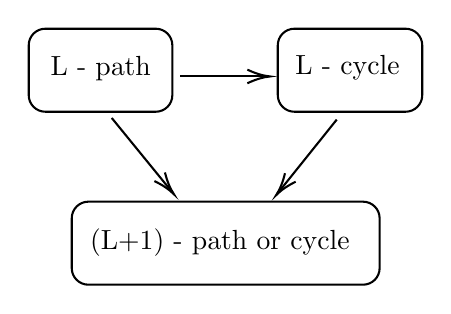
\begin{tikzpicture}[x=0.75pt,y=0.75pt,yscale=-1,xscale=1]
    %uncomment if require: \path (0,300); %set diagram left start at 0, and has height of 300

    %Rounded Rect [id:dp2247988663004169] 
    \draw   (100.6,84) .. controls (100.6,79.58) and (104.18,76) .. (108.6,76) -- (161.8,76) .. controls (166.22,76) and (169.8,79.58) .. (169.8,84) -- (169.8,108) .. controls (169.8,112.42) and (166.22,116) .. (161.8,116) -- (108.6,116) .. controls (104.18,116) and (100.6,112.42) .. (100.6,108) -- cycle ;
    %Rounded Rect [id:dp3322171879942837] 
    \draw   (220.6,84) .. controls (220.6,79.58) and (224.18,76) .. (228.6,76) -- (282.2,76) .. controls (286.62,76) and (290.2,79.58) .. (290.2,84) -- (290.2,108) .. controls (290.2,112.42) and (286.62,116) .. (282.2,116) -- (228.6,116) .. controls (224.18,116) and (220.6,112.42) .. (220.6,108) -- cycle ;
    %Rounded Rect [id:dp522325016929076] 
    \draw   (121.33,167.33) .. controls (121.33,162.92) and (124.92,159.33) .. (129.33,159.33) -- (261.67,159.33) .. controls (266.08,159.33) and (269.67,162.92) .. (269.67,167.33) -- (269.67,191.33) .. controls (269.67,195.75) and (266.08,199.33) .. (261.67,199.33) -- (129.33,199.33) .. controls (124.92,199.33) and (121.33,195.75) .. (121.33,191.33) -- cycle ;
    %Straight Lines [id:da4471732816066223] 
    \draw    (173.53,99) -- (214.87,99) ;
    \draw [shift={(216.87,99)}, rotate = 180] [color={rgb, 255:red, 0; green, 0; blue, 0 }  ][line width=0.75]    (10.93,-3.29) .. controls (6.95,-1.4) and (3.31,-0.3) .. (0,0) .. controls (3.31,0.3) and (6.95,1.4) .. (10.93,3.29)   ;
    %Straight Lines [id:da08077221270601986] 
    \draw    (140.6,119) -- (169.34,154.25) ;
    \draw [shift={(170.6,155.8)}, rotate = 230.81] [color={rgb, 255:red, 0; green, 0; blue, 0 }  ][line width=0.75]    (10.93,-3.29) .. controls (6.95,-1.4) and (3.31,-0.3) .. (0,0) .. controls (3.31,0.3) and (6.95,1.4) .. (10.93,3.29)   ;
    %Straight Lines [id:da17940502186011487] 
    \draw    (249,119.8) -- (221.05,154.64) ;
    \draw [shift={(219.8,156.2)}, rotate = 308.74] [color={rgb, 255:red, 0; green, 0; blue, 0 }  ][line width=0.75]    (10.93,-3.29) .. controls (6.95,-1.4) and (3.31,-0.3) .. (0,0) .. controls (3.31,0.3) and (6.95,1.4) .. (10.93,3.29)   ;

    % Text Node
    \draw (109.6,87.67) node [anchor=north west][inner sep=0.75pt]   [align=left] {L - path};
    % Text Node
    \draw (227.6,87.27) node [anchor=north west][inner sep=0.75pt]   [align=left] {L - cycle};
    % Text Node
    \draw (128.67,171) node [anchor=north west][inner sep=0.75pt]   [align=left] {(L+1) - path or cycle};


    \end{tikzpicture}
\end{center}

\section{Path of length $l$}

Let $P = \{x_1, e_1, x_2, e_2, \dots, x_{l}, e_{l}, x_{l + 1}\}$ be a $l$ length path. Let's define some variables that will
be used in the algorithm:

\begin{itemize}
    \item $G$ - Collection of graphs
    \item $n$ - Size of $G$ and number of vertices in $G_i$
    \item $colors\_in\_path$ - Array of size $n$ where $colors\_in\_path[i]$ is True if color $i$ is in the set of colors of the edges of the path
    \item $vertices\_in\_path$ - Array of size $n$ where $vertices\_in\_path[i]$ is True if vertex $i$ is in the path
\end{itemize}

\subsection{$l \leq \left \lceil \frac{n}{2} \right \rceil$}

Take a color $c$ that is not in the set of colors of the edges of the path. As $deg(x_{l + 1}, c) >= \left \lceil \frac{n}{2} \right \rceil$
and there are at most $l < \left \lceil \frac{n}{2} \right \rceil$ other vertices on the path, then there exists a 
vertex $y$ outside the path such that $y$ is adjacent to $x_{l + 1}$ and $\{y, x_{l + 1}\} \in E(G_c)$.

\begin{algorithm}
    \caption{Pseudocódigo para verificar caminho}
    \begin{algorithmic}[1]
        \Function{Increment\_Path\_Small\_Case}{$G, P$}
        \State \textbf{Assert}($P.\text{size()} < \lceil \frac{n}{2} \rceil + 1$)
        \State $vertices \gets P.\text{vertices}$
        \State $edges \gets P.\text{edges}$
        \State $final\_vertex \gets P.\text{back()}$
        \For{$color \in \{0, \dots, n-1\}$}
            \If{\textbf{not} $colors\_in\_path[color]$}
                \For{$i \in \{0, \dots, n-1\}$}
                    \If{\textbf{not} $vertices\_in\_path[i]$}
                        \State $edge \gets G.\text{check\_edge}(final\_vertex, i, color)$
                        \If{$edge \neq \text{None}$}
                            \State $vertices.\text{append}(i)$
                            \State $edges.\text{append}(edge)$
                            \State \Return Path($G$, $vertices$, $edges$)
                        \EndIf
                    \EndIf
                \EndFor
            \EndIf
        \EndFor
        \State \textbf{Assert}(False, Should not reach here.)
    \EndFunction
    \end{algorithmic}
\end{algorithm}


\section{Cycle of length $n - 1 \neq \ell \geq \left \lfloor \frac{n}{2} \right \rfloor$}

\section{Cycle of length $n - 1$}


